% !TeX program = pdflatex
% !TeX spellcheck = en_US
% !TeX encoding = UTF-8

% update
% v1.13 - 2020-01-15
% - Tanja: change the style.tex: define Black as a color and use it to replace DarkRed (except on the title page)
% - Tanja: change the the titlepage once more 
% - Tanja: change the color code for DarkRed to match the current TU logo sytle
% v1.12 - 2020-01-02
% - Tanja: add new titlepage design and replace all logos with the new one
% v1.11 - 2018-10-15
% - Felix: use Bibtex instead of Biblatex
% v1.10 - 2017-05-30
% - Erik: Refactor the file structure of the front pages
% - Erik: Fix double bibliography entry
% v1.9 - 2017-02-03
% - Dirk: fixed warning: Underfull \hbox (badness 10000) in paragraph main.tex
% - Dirk: fixed warning: "Data encoding is UTF8" -> style.tex 0.1.8
% v1.8 - 2017-02-02
% - Dirk: replaced titlesec package by KOMA-script commands.-> style.tex v0.1.7
% v1.7 - 2014-11-18
% - bib fixes: now using biber instead of bibtex (thanks felix)
% - compile now with pdflatex -> biber -> pdflatex
% v1.6 - 2013-05-13
% - bibliography headers fixed - thanx lorenz lehmann
% - high quality titlepage - thanx thomas graf
% - removed separation of online and offline references -> style 1.4a
% v1.5 - 2013-01-16

\documentclass[twoside,11pt,titlepage,a4paper,english,bibliography=totocnumbered,listof=numbered]{scrbook}
%
% Template Style
% =========================================================================
% = SNET THESIS TEMPLATE STYLE
% =========================================================================

% http://www.snet.tu-berlin.de
% ------------------------
% Adapted version from http://hci.rwth-aachen.de/karrer_thesistemplate (Thorsten Karrer)
% Further adaptions for http://www.elearn.rwth-aachen.de (Sascha Hoellger)
% Further adaptions for SNET @ TU Berlin by Sebastian Göndör (sebastian.goendoer@tu-berlin.de)


% =========================================================================
% = CHANGELOG
% =========================================================================
% [0.1.9]
% - Fixed styling for chapters and toc using Komascript
% - Remove double bibliography TOC entry
%
% [0.1.8]
% - fixed "warning UFT8 is used". biblatex requires ascii encoding; by Dirk
%
% [0.1.7]
% replaced "Titelsec" commands (and whole package) by appropriate KOMA-Script commands; by Dirk
%
% [0.1.6]
% replaced deprecated \rm commands with \rmfamily commands; by Dirk
%
% [0.1.4b]
% backend=biber added in line 139
%
% [0.1.4a]
% title page: image logo sizes and margins adjusted to printable area
% removed separation of online and offline references
%
% [0.1.3]
% wider text body
% added "school" to the titlepage
% paragraph indents
% correctly placed footnote graphics
%
% [0.1.2]
% new titlepage
% some minor fixes
%
% [0.1.1]
% changed titlepage logo
% added listoffigures and listoftables
% excluded abstract from toc
% no (roman) numbering for frontmatter
%
% [0.1]
% adapted version 0.991b from sascha hoellger @ rwth aachen


% =========================================================================
% = MISC
% =========================================================================

\usepackage{a4wide}					%
\usepackage{verbatim}				%
\usepackage[toc,page]{appendix}			%
\usepackage[withpage]{acronym}			%
\usepackage{amsthm}				% Definitions


% =========================================================================
% = COLORS
% =========================================================================

\usepackage{xcolor}					% Colors
\definecolor{LightBlue}{rgb}{0.55,0.55,1}
\definecolor{DarkBlue}{rgb}{0.2,0.2,0.5}
\definecolor{DarkRed}{rgb}{0.7725490196,0.05490196078,0.12549019607} % new TU red
\definecolor{Black}{rgb}{0,0,0}

% =========================================================================
% = PAGE LAYOUT
% =========================================================================

\usepackage{geometry}
\geometry{inner=3cm, outer=2cm, bottom=4cm}

\newcommand{\setwidesite}				% changes the geometry to have less margin
{
	\fancyhfoffset[LE,RO]{0cm}
	\fancyheadoffset[LO,RE]{0cm}
	\fancyfootoffset[RE]{2cm}
	\newgeometry{inner=2cm, outer=2cm, bottom=4cm}
}

\usepackage{style/noindent}				%do not indent at new paragraphs but add a vertical offset

\setlength{\parindent}{4mm}
\setlength{\parskip}{1.5mm }


% =========================================================================
% = TYPESETTING
% =========================================================================

\usepackage[hyphens]{url}				% url
\usepackage{hyphenat}				% hyphenation. use \hyphenation{}

\righthyphenmin=5
\lefthyphenmin=5


% =========================================================================
% = TABLE OF CONTENTS
% =========================================================================

\setcounter{secnumdepth}{4}
\setcounter{tocdepth}{3}

\addtokomafont{disposition}{\rmfamily}


% =========================================================================
% = FONTS
% =========================================================================

\usepackage{mathpazo}
\usepackage[scaled=.95]{helvet}
\usepackage{courier}


% =========================================================================
% = SYMBOLS
% =========================================================================

%\usepackage{gensymb}
\usepackage{textcomp} 				% for \textmu (non-italic $\mu$)
\makeatletter						% this makes "@" a regular letter


% =========================================================================
% = TABLES
% =========================================================================

\usepackage{tabularx}
\usepackage{booktabs}
\usepackage{multirow}
\usepackage{longtable}				% tables spanning over more than one page

%%\setlength{\fboxsep}{0mm}			% spacing between \fbox border and content

\usepackage{amsmath}				% math fonts
\usepackage{amssymb}				% math symbols
\usepackage{setspace}				% line spacing


% =========================================================================
% = BIBILOGRAPHY
% =========================================================================

% 2018-10-16 - changed to use Bibtex instead

%\usepackage[style=numeric,natbib=true,backend=biber]{biblatex}

% apparently no effect?
%\renewcommand{\bibsetup}{
%	\markboth{
%		\MakeUppercase{Bibliography}
%	}{}
%}

%\ifdefined\bibheadingonline
%  \defbibheading{online}{\section*{\bibheadingonline}}
%\else
%  \defbibheading{online}{\section*{Online References}}
%\fi
%\ifdefined\bibheadingoffline
%  \defbibheading{offline}{\section*{\bibheadingoffline}}
%\else
%  \defbibheading{offline}{\section*{Printed References}}
%\fi
%
%\defbibfilter{online}{%
%  \( \type{online} \)}
%
%\defbibfilter{offline}{%
%  \( \not \type{online} \)}
%
%\bibliography{Bibliography}


% =========================================================================
% = LANGUAGE & ENCODING
% =========================================================================

\usepackage[english]{babel}				% \usepackage[ngerman]{babel}

\selectlanguage{english}				% \selectlanguage{ngerman}

\usepackage[T1]{fontenc}
\usepackage[utf8]{inputenc}				% can use native umlauts

% \usepackage[babel,german=quotes]{csquotes}	% provides \enquote{Blupp} => "`Blupp"'
\usepackage[babel,english=american]{csquotes}	% provides \enquote{Blupp} => "`Blupp"'

%\SetCiteCommand{\parencite}			% Changed for biblatex

\usepackage{units}					% unified way of setting values with units

\usepackage{appendix}


% =========================================================================
% = CODE LISTINGS
% =========================================================================

\usepackage{listings}

% Listings Styles from Max

\definecolor{violet}{cmyk}{0.45,0.97,0.27,0.21}
\definecolor{lstblue}{cmyk}{1,0.80,0,0}
\definecolor{lstgreen}{cmyk}{0.71,0.21,0.65,0.22}
\definecolor{bluegrey}{cmyk}{0.56,0.24,0.11,0.05}
\definecolor{javadoc}{cmyk}{0.88,0.59,0,0}
\definecolor{lstgrey}{cmyk}{0.55,0.44,0.42,0.32}

\lstdefinelanguage{SQL}{
     keywords={},
     keywordstyle=\color{bluegrey}\bfseries,
     morekeywords=[2]{CREATE,TABLE,IF,NOT,EXISTS,NULL,SET,DEFAULT,PRIMARY,KEY,COLLATE,CHARACTER,AUTO_INCREMENT,ENGINE,CHARSET},
     keywordstyle={[2]\color{violet}\bfseries},
     otherkeywords={int,varchar,double,text,tinyint},
     sensitive=false,
     morecomment=[l][\color{lstgreen}]{//},
     morecomment=[s][\color{lstgreen}]{/*}{*/},
     morecomment=[s][\color{javadoc}]{/**}{*/},
     morestring=[b]',
     morestring=[b]"
  }
\lstdefinelanguage{PHP}{
     keywords={},
     keywordstyle=\color{bluegrey}\bfseries,
     morekeywords=[2]{static,function,if,return,pow,sin,cos,asin,min,sqrt,int},
     keywordstyle={[2]\color{violet}\bfseries},
     otherkeywords={@param, @returns, @author, @type, @link, @see},
     sensitive=false,
     morecomment=[l][\color{lstgreen}]{//},
     morecomment=[s][\color{lstgreen}]{/*}{*/},
     morecomment=[s][\color{javadoc}]{/**}{*/},
     morestring=[b]',
     morestring=[b]"
  }
\lstdefinelanguage{JavaScript}{
     keywords={},
     keywordstyle=\color{bluegrey}\bfseries,
     morekeywords=[2]{attributes, class, classend, do, empty, endif, endwhile, fail, function, functionend, if, implements, in, inherit, inout, not, of, operations, out, return, set, then, types, while, use},
     keywordstyle={[2]\color{violet}\bfseries},
     otherkeywords={@param, @returns, @author, @type, @link, @see},
     sensitive=false,
     morecomment=[l][\color{lstgreen}]{//},
     morecomment=[s][\color{lstgreen}]{/*}{*/},
     morecomment=[s][\color{javadoc}]{/**}{*/},
     morestring=[b]',
     morestring=[b]"
  }
\lstdefinelanguage{Java}{
     keywords={},
     keywordstyle=\color{bluegrey}\bfseries,
     morekeywords=[2]{abstract,boolean,break,byte,case,catch,char,class,
      const,continue,default,do,double,else,extends,false,final,
      finally,float,for,goto,if,implements,import,instanceof,int,
      interface,label,long,native,new,null,package,private,protected,
      public,return,short,static,super,switch,synchronized,this,throw,
      throws,transient,true,try,void,volatile,while},
     keywordstyle={[2]\color{violet}\bfseries},
     morekeywords=[3]{@SuppressWarnings, @Capability, @Override},
     keywordstyle={[3]\color{lstgrey}},
     otherkeywords={@param, @return, @returns, @author, @link, @see},
     sensitive,
     morecomment=[l]//,
     morecomment=[s]{/*}{*/},
     morecomment=[s][\color{javadoc}]{/**}{*/},
     morestring=[b]",
     morestring=[b]',
  }[keywords,comments,strings]

% some listings styles from Gregor Aisch
% http://vis4.net/blog/2009/09/noch-mehr-sprach-definitionen-fuer-latex-listings/

\lstdefinelanguage{HTML5} {morekeywords={a, abbr, address, area, article, aside, audio, b, base, bb, bdo, blockquote,  body, br, button, canvas, caption, cite, code, col, colgroup, command, datagrid, datalist, dd, del, details, dialog, dfn, div, dl, dt, em, embed, eventsource, fieldset, figure, footer,  form,  h1, h2,  h3,  h4, h5,  h6,  head,  header,  hr, html,  i, iframe,  img,  input,  ins, kbd,  label,  legend,  li,  link,  mark,  map,  menu,  meta,  meter,  nav,  noscript,  object,  ol,  optgroup,  option,  output,  p,  param,  pre,  progress,  q,  ruby,  rp,  rt,  samp,  script,  section,  select,  small,  source,  span,  strong,  style,  sub,  sup,  table,  tbody,  td,  textarea,  tfoot,  th,  thead,  time,  title,  tr,  ul,  var,  video},
sensitive=false, morecomment=[s]{<!--}{-->}, morestring=[b]", morestring=[d]'}

\lstdefinelanguage{CSS} {morekeywords={azimuth,  background-attachment,  background-color,  background-image,  background-position,  background-repeat,  background,  border-collapse,  border-color,  border-spacing,  border-style,  border-top, border-right, border-bottom, border-left,  border-top-color, border-right-color, border-bottom-color, border-left-color,  border-top-style, border-right-style, border-bottom-style, border-left-style,  border-top-width, border-right-width, border-bottom-width, border-left-width,  border-width,  border,  bottom,  caption-side,  clear,  clip,  color,  content,  counter-increment,  counter-reset,  cue-after,  cue-before,  cue,  cursor,  direction,  display,  elevation,  empty-cells,  float,  font-family,  font-size,  font-style,  font-variant,  font-weight,  font,  height,  left,  letter-spacing,  line-height,  list-style-image,  list-style-position,  list-style-type,  list-style,  margin-right, margin-left,  margin-top, margin-bottom,  margin,  max-height,  max-width,  min-height,  min-width,  orphans,  outline-color,  outline-style,  outline-width,  outline,  overflow,  padding-top, padding-right, padding-bottom, padding-left,  padding,  page-break-after,  page-break-before,  page-break-inside,  pause-after,  pause-before,  pause,  pitch-range,  pitch,  play-during,  position,  quotes,  richness,  right,  speak-header,  speak-numeral,  speak-punctuation,  speak,  speech-rate,  stress,  table-layout,  text-align,  text-decoration,  text-indent,  text-transform,  top,  unicode-bidi,  vertical-align,  visibility,  voice-family,  volume,  white-space,  widows,  width,  word-spacing,  z-index},
sensitive=false, morecomment=[s]{/*}{*/}, morestring=[b]", morestring=[d]'}

\lstdefinelanguage{JavaFX} {morekeywords={abstract, after, and, as, assert, at, attribute, before, bind, bound, break, catch, class, continue, def, delete, else, exclusive, extends, false, finally, first, for, from, function, if, import, indexof, in, init, insert, instanceof, into, inverse, last, lazy, mixin, mod, new, not, null, on, or, override, package, postinit, private, protected, public-init, public, public-read, replace, return, reverse, sizeof, static, step, super, then, this, throw, trigger, true, try, tween, typeof, var, where, while, with },
sensitive=false, morecomment=[l]{//}, morecomment=[s]{/*}{*/}, morestring=[b]", morestring=[d]'}

\lstdefinelanguage{MXML} {morekeywords={mx:Accordion, mx:Box, mx:Canvas, mx:ControlBar, mx:DividedBox, mx:Form, mx:FormHeading, mx:FormItem, mx:Grid, mx:GridItem, mx:GridRow, mx:HBox, mx:HDividedBox, mx:LinkBar, mx:Panel, mx:TabBar, mx:TabNavigator, mx:Tile, mx:TitleWindow, mx:VBox, mx:VDividedBox, mx:ViewStack, mx:Button, mx:CheckBox, mx:ComboBase, mx:ComboBox, mx:DataGrid, mx:DateChooser, mx:DateField, mx:HRule, mx:Image, mx:Label, mx:Link, mx:List, mx:Loader, mx:MediaController, mx:MediaDisplay, mx:MediaPlayback, mx:MenuBar, mx:NumericStepper, mx:ProgressBar, mx:RadioButton, mx:RadioButtonGroup, mx:Spacer, mx:Text, mx:TextArea, mx:TextInput, mx:Tree, mx:VRule, mx:VScrollBar, mx:Application, mx:Repeater, mx:UIComponent, mx:UIObject, mx:View, mx:FlexExtension, mx:UIComponentExtension, mx:UIObjectExtension, mx:Fade, mx:Move, mx:Parallel, mx:Pause, mx:Resize, mx:Sequence, mx:WipeDown, mx:WipeLeft, mx:WipeRight, mx:WipeUp, mx:Zoom, mx:EventDispatcher, mx:LowLevelEvents, mx:UIEventDispatcher, mx:CurrencyFormatter, mx:DateFormatter, mx:NumberFormatter, mx:PhoneFormatter, mx:ZipCodeFormatter, mx:CursorManager, mx:DepthManager, mx:DragManager, mx:FocusManager, mx:HistoryManager, mx:LayoutManager, mx:OverlappedWindows, mx:PopUpManager, mx:SystemManager, mx:TooltipManager, mx:CreditCardValidator, mx:DateValidator, mx:EmailValidator, mx:NumberValidator, mx:PhoneNumberValidator, mx:SocialSecurityValidator, mx:StringValidator, mx:ZipCodeValidator, mx:DownloadProgressBar, mx:ArrayUtil, mx:ClassUtil, mx:Delegate, mx:ObjectCopy, mx:URLUtil, mx:XMLUtil, mx:CSSSetStyle, mx:CSSStyleDeclaration, mx:CSSTextStyles, mx:StyleManager, mx:HTTPService, mx:RemoteObject, mx:Service},
sensitive=false, morecomment=[s]{<!--}{-->}, morestring=[b]", morestring=[d]'}

\lstdefinelanguage{LZX} {morekeywords={a, alert, animator, animatorgroup , attribute, audio , axis, axisstyle , b, barchart, basebutton , basebuttonrepeater , basecombobox , basecomponent , basedatacombobox , basedatepicker , basedatepickerday , basedatepickerweek , basefloatinglist , basefocusview , baseform , baseformitem , basegrid , basegridcolumn , baselist , baselistitem , basescrollarrow , basescrollbar , basescrollthumb , basescrolltrack , baseslider , basestyle , basetab , basetabelement , basetabpane , basetabs , basetabsbar , basetabscontent , basetabslider , basetrackgroup , basetree , basevaluecomponent , basewindow , br , button , canvas , chart , chartbgstyle , chartstyle , checkbox , class , columnchart , combobox , command , connection , connectiondatasource , constantboundslayout , constantlayout , datacolumn , datacombobox , datalabel , datamarker , datapath , datapointer , dataselectionmanager , dataseries , dataset , datasource , datastyle , datastylelist , datatip , datepicker , debug , dragstate , drawview , edittext , event , face , floatinglist , font , font , form , frame , grid , gridcolumn , gridtext , handler , hbox , horizontalaxis , hscrollbar , i , image , img , import , include , inputtext , javarpc , label , labelstyle , layout , legend , library , linechart , linestyle , list , listitem , LzTextFormat , menu , menubar , menuitem , menuseparator , method , modaldialog , multistatebutton , node , p , param , piechart , piechartplotarea , plainfloatinglist , plotstyle , pointstyle , pre , radiobutton , radiogroup , rectangularchart , regionstyle , remotecall , resizelayout , resizestate , resource , reverselayout , richinputtext , rpc , script , scrollbar , security , selectionmanager , sessionrpc , simpleboundslayout , simpleinputtext , simplelayout , slider , soap , splash , stableborderlayout , state , statictext , style , submit , swatchview , SyncTester , tab , tabelement , tabpane , tabs , tabsbar , tabscontent , tabslider , Test , TestCase , TestResult , TestSuite , text , textlistitem , tickstyle , tree , u , valueline , valuelinestyle , valuepoints , valuepointstyle , valueregion , valueregionstyle , vbox , verticalaxis , view , view , vscrollbar , webapprpc , window , windowpanel , wrappinglayout , XMLHttpRequest , xmlrpc , zoomarea},
sensitive=false, morecomment=[s]{<!--}{-->}, morestring=[b]", morestring=[d]'}

\lstset{
  numbers=left,
  numberstyle=\tiny,
  numbersep=5pt,
  breaklines=true,
  stepnumber=1,
  tabsize=2,
  basicstyle=\ttfamily\small,
  frame=none,
  numberfirstline=true,
  firstnumber=1,
  keywordstyle=\color{violet}\bfseries,
  ndkeywordstyle=\color{bluegrey}\bfseries,
  identifierstyle=\color{black},
  commentstyle=\color{lstgreen}\ttfamily,
  stringstyle=\color{lstblue}\ttfamily,
  showstringspaces=false
}


% ========================================================================
% = CHANGE LIST DEFINITIONS
% ========================================================================

% change color of item list
\renewcommand{\labelitemi}{\color{Black}$\bullet$}
\renewcommand{\labelitemii}{\color{Black}$\circ$}
\renewcommand{\labelitemiii}{\color{Black}$\ast$}
\renewcommand{\labelitemiv}{\color{Black}$\diamond$}

% change color of enum list
\renewcommand{\labelenumi}{\color{Black}\arabic{enumi}.}
\renewcommand{\labelenumii}{\color{Black}\alph{enumii})}
\renewcommand{\labelenumiii}{\color{Black}\roman{enumiii}.}
\renewcommand{\labelenumiv}{\color{Black}\Alph{enumiv}.}

% change color of description list
\usepackage{enumitem}
\setdescription{font=\color{Black}\rmfamily\itshape}
%\renewenvironment{description}{\list{font=\color{Black}\itshape}}{\endlist}


% ========================================================================
% = FOOTNOTES
% ========================================================================

% change color of footnotes
\renewcommand{\thefootnote}{\color{Black}\arabic{footnote}}

% use nice footnote indentation
\deffootnote[1em]{1em}{1em}{\textsuperscript{\thefootnotemark}\,}


% =========================================================================
% = GRAPHICS AND IMAGES
% =========================================================================

\usepackage{graphicx}
\graphicspath{{images/}}				% path to your image folder

\usepackage{eso-pic}					% needed for the full-face titlepage
\usepackage{chngpage}				% we need this to determine if a figure is on an odd or even page
\usepackage{tikz}					% tikz pictures

% captions of tables and images
\usepackage[hang,small,sf]{caption}
\renewcommand{\captionfont}{\sffamily\small}
\renewcommand{\captionlabelfont}{\bfseries}

\usepackage{float}
\usepackage{placeins}
% \floatstyle{ruled}
%\floatplacement

\renewcommand{\floatpagefraction}{0.85}		% if a figure takes more than 85% of a page it will be typeset on a separate page
\usepackage[it,bf,tight,hang,raggedright]{subfigure}

%\numberwithin{figure}{section}
%\numberwithin{table}{section}


% =========================================================================
% = HEADER
% =========================================================================

\newcommand{\STYLEfootnotetext}
%{
%  \begin{minipage}
%  {.2\textwidth}
%    \includegraphics[width=0.6\textwidth]{images/snet/snet_footer.png}
%  \end{minipage}
%}

% Change page headers and footers:
\usepackage{calc}
\usepackage{fancyhdr}
\pagestyle{fancy}
\fancyhfoffset[RO,LE]{0.1cm} %{\marginparsep+\marginparwidth}
\fancyhfoffset[RE,LO]{0.1cm}
%\fancyheadoffset[RE,LO]{\hoffset + \oddsidemargin}
\renewcommand{\headrule}{{\color{Black}%
  \hrule width\headwidth height\headrulewidth \vskip-\headrulewidth}}
\fancyhf{}
\fancyhead[RE]{\slshape \nouppercase{\leftmark}}    % Even page header: "page   chapter"
\fancyhead[LO]{\slshape \nouppercase{\rightmark}}   % Odd  page header: "section   page"
\fancyhead[RO,LE]{\bfseries \thepage}

%- \fancyfoot[LE]{\STYLEleftpicture}
%- \fancyfoot[RO]{\STYLErightpicture}
\fancyfoot[LE]{\STYLEfootnotetext}

\renewcommand{\headrulewidth}{1pt}    % Underline headers
\renewcommand{\footrulewidth}{0pt}

% =========================================================================
% = SECTIONS THEMING
% =========================================================================

\newcommand{\allsectionformat}{\color{Black}\rmfamily\normalfont}

% Font style and colors
\addtokomafont{part}{\Huge\allsectionformat}
\addtokomafont{chapter}{\Huge\allsectionformat}
\addtokomafont{section}{\allsectionformat}
\addtokomafont{subsection}{\allsectionformat}
\addtokomafont{subsubsection}{\allsectionformat}
\addtokomafont{paragraph}{\allsectionformat}
\addtokomafont{subparagraph}{\allsectionformat}

% Spacing before and after the section titles
\RedeclareSectionCommand[
  beforeskip=-.75\baselineskip,
  afterskip=.5\baselineskip]{section}

\RedeclareSectionCommand[
  beforeskip=-5\baselineskip,
  afterskip=.5\baselineskip]{chapter}


% =========================================================================
% = TYPESETTING - TWEAKES
% =========================================================================

\addtokomafont{section}{\LARGE}
\addtokomafont{subsection}{\large}

% instead of sloppy
%\tolerance 1414
%\hbadness 1414
%- \tolerance 2414
%- \hbadness 2414
%- \emergencystretch 1.5em
%- \hfuzz 0.3pt
%- \widowpenalty=10000
%- \clubpenalty=10000
%- \brokenpenalty=10000
%- \interlinepenalty=9000 % seitenumbruch im absatz
%- \vfuzz \hfuzz
%- \raggedbottom


% =========================================================================
% =  USER DEFINED COMMANDS
% =========================================================================

\newcommand{\chapterquote}[2]{
    \begin{quotation}
    \begin{flushright}
    \noindent\emph{``{#1}''\\[1.5ex]---{#2}}
    \end{flushright}
    \end{quotation}
}

% Copyright 2017 Sergei Tikhomirov, MIT License
% https://github.com/s-tikhomirov/solidity-latex-highlighting/

\usepackage{listings, xcolor}

\definecolor{verylightgray}{rgb}{.97,.97,.97}

\lstdefinelanguage{Solidity}{
	keywords=[1]{anonymous, assembly, assert, balance, break, call, callcode, case, catch, class, constant, continue, constructor, contract, debugger, default, delegatecall, delete, do, else, emit, event, experimental, export, external, false, finally, for, function, gas, if, implements, import, in, indexed, instanceof, interface, internal, is, length, library, log0, log1, log2, log3, log4, memory, modifier, new, payable, pragma, private, protected, public, pure, push, require, return, returns, revert, selfdestruct, send, solidity, storage, struct, suicide, super, switch, then, this, throw, true, try, typeof, using, value, view, while, with, addmod, ecrecover, keccak256, mulmod, ripemd160, sha256, sha3}, % generic keywords including crypto operations
	keywordstyle=[1]\color{blue}\bfseries,
	keywords=[2]{address, bool, byte, bytes, bytes1, bytes2, bytes3, bytes4, bytes5, bytes6, bytes7, bytes8, bytes9, bytes10, bytes11, bytes12, bytes13, bytes14, bytes15, bytes16, bytes17, bytes18, bytes19, bytes20, bytes21, bytes22, bytes23, bytes24, bytes25, bytes26, bytes27, bytes28, bytes29, bytes30, bytes31, bytes32, enum, int, int8, int16, int24, int32, int40, int48, int56, int64, int72, int80, int88, int96, int104, int112, int120, int128, int136, int144, int152, int160, int168, int176, int184, int192, int200, int208, int216, int224, int232, int240, int248, int256, mapping, string, uint, uint8, uint16, uint24, uint32, uint40, uint48, uint56, uint64, uint72, uint80, uint88, uint96, uint104, uint112, uint120, uint128, uint136, uint144, uint152, uint160, uint168, uint176, uint184, uint192, uint200, uint208, uint216, uint224, uint232, uint240, uint248, uint256, var, void, ether, finney, szabo, wei, days, hours, minutes, seconds, weeks, years},	% types; money and time units
	keywordstyle=[2]\color{teal}\bfseries,
	keywords=[3]{block, blockhash, coinbase, difficulty, gaslimit, number, timestamp, msg, data, gas, sender, sig, value, now, tx, gasprice, origin},	% environment variables
	keywordstyle=[3]\color{violet}\bfseries,
	identifierstyle=\color{black},
	sensitive=true,
	comment=[l]{//},
	morecomment=[s]{/*}{*/},
	commentstyle=\color{gray}\ttfamily,
	stringstyle=\color{red}\ttfamily,
	morestring=[b]',
	morestring=[b]"
}

\lstset{
	language=Solidity,
	%backgroundcolor=\color{verylightgray},
	extendedchars=true,
	basicstyle=\footnotesize\ttfamily,
	showstringspaces=false,
	showspaces=false,
	numbers=left,
	numberstyle=\footnotesize,
	numbersep=9pt,
	tabsize=2,
	breaklines=true,
	showtabs=false,
	captionpos=b,
        frame=single
}

\lstset{prebreak=\raisebox{0ex}[0ex][0ex]
        {\ensuremath{\rhookswarrow}}}
\lstset{postbreak=\raisebox{0ex}[0ex][0ex]
        {\ensuremath{\rcurvearrowse\space}}}
\lstset{breaklines=true, breakatwhitespace=true}
\lstset{numbers=left, numberstyle=\scriptsize}

% custom hyphenation					% add words to this list to prevent hyphenation
\hyphenation{
ASCII
TCP
}

%make readable references
\usepackage[pdftex,pdfpagelabels=true]{hyperref}
\usepackage[acronym]{glossaries}
\usepackage{MnSymbol}
\usepackage{booktabs}
\usepackage{tabularx}
\usepackage{xltabular}
\hypersetup{%
	pdftitle={Thesis Title},
	pdfauthor={Thesis Author},
	pdfkeywords={key1, key2, key3},
	pdfsubject={Thesis Subject}
}

% Adding a finite stretch on the page suppresses "Underfull \vbox (badness 10000)" warnings.
\makeatletter
\def\@textbottom{\vskip \z@ \@plus 1pt}
\let\@texttop\relax
\makeatother
\makeglossaries
\newacronym{zb}{ZB}{Zettabytes}
\newacronym{iot}{IoT}{Internet of Things}
\newacronym{spof}{SPOF}{Single Point of Failure}
\newacronym{pii}{PII}{Personal Identifiable Information}
\newacronym{gdpr}{GDPR}{European General Data Protection Regulation}
\newacronym{ttp}{TTP}{Trusted Third Party}
\newacronym{zkp}{ZKP}{Zero-knowledge Proof}
\newacronym{nizkp}{NIZKP}{Non-interactive Zero-knowledge Proof}
\newacronym{zksnark}{ZK-SNARK}{Zero-Knowledge Succinct Non-Interactive Argument of Knowledge}
\newacronym{csr}{CRS}{Common Reference String}
\newacronym{smpc}{MPC/SMPC}{Secure Multi-Party Computation}
\newacronym{ecdsa}{ECDSA}{Elliptic Curve Digital Signature Algorithm}
\newacronym{dlp}{DLP}{Discrete Logarithm Problem}
\newacronym{zksnork}{ZK-SNORK}{Succinct Non-interactive Oecumenical (Universal) aRguments of Knowledge}
\newacronym{zkstark}{ZK-STARK}{Zero-Knowledge Scalable Transparent Argument of Knowledge}
\newacronym{evm}{EVM}{Ethereum Virtual Machine}
\newacronym{ringct}{RingCT}{Ring Confidential Transaction}
\newacronym{srs}{SRS}{Structured Reference String}
\newacronym{voc}{VOC}{Verifiable Off-chain Computation}
\newacronym{dos}{DoS}{Denial of Service}
\newacronym{eoa}{EOA}{Externally Owned Account}
\newacronym{eip20}{EIP-20}{Ethereum Improvement Proposal 20}
\newacronym{eip721}{EIP-721}{Ethereum Improvement Proposal 721}
\newacronym{erc20}{ERC-20}{Ethereum Request for Comments 20}
\newacronym{erc721}{ERC-721}{Ethereum Request for Comments 721}
\newacronym{nft}{NFT}{Non-Fungible Token}
\newacronym{ioc}{IOC}{Incentive-driven Off-chain Computing}
\newacronym{tee}{TEE}{Trusted Execution Environment}
\newacronym{he}{HE}{Homomorphic Encryption}
\newacronym{dp}{DP}{Differential Privacy}
\newacronym{fe}{FE}{Functional Encryption}
\newacronym{hibe}{HIBE}{Hierarchical Identity-Based Encryption}

\begin{document}

%--------------------------------------------------------------
% FRONT PAGE AND DOCUMENT METADATA
%--------------------------------------------------------------
\frontmatter

\newgeometry{centering}
\begin{titlepage}
\AddToShipoutPicture*{
    \put(0,0){
        
\includegraphics[width=\paperwidth,height=\paperheight,keepaspectratio=false]{images/snet/titlepage_ise.pdf}
    }
}
\strut
\hfill
\begin{center}
\vspace{1cm}
    \Huge
    \begin{spacing}{.9}
        \textbf{Enabling Compute-to-Data through Verifiable Off-Chain Computations for Blockchain-based Data Trading}\\
    \end{spacing}
    \vspace{0.8cm}
    \large
    by\\
    \vspace{0.8cm}
    \textbf{Kevin Hertwig}\\
    \vspace{0.8cm}
    \textbf{Matriculation Number 388430}\\
    \vspace{1.4cm}
    A thesis submitted to\\
    \vspace{0.5cm}
    Technische Universität Berlin\\
    Faculty IV - Electrical Engineering and Computer Science\\
    Business Informatics - Commercial Information Technology and Quantitative Methods\\
    Information Systems Engineering\\
    \vspace{0.5cm}
    \textbf{Master's Thesis}\\
    \vspace{1.4cm}
    \today\\
    \vspace{1.4cm}
    \large
    Supervised by:\\
    Prof. Dr.-Ing. Stefan Tai\\
    \vspace{1cm}
    Assistant supervisor:\\
    Prof. Dr. Axel Küpper\\
    \end{center}
\end{titlepage}
\restoregeometry

% Clear two pages after the title
\shipout\null
\shipout\null

\chapter*{\LARGE Eidestattliche Erklärung / Statutory Declaration}
Hiermit erkläre ich, dass ich die vorliegende Arbeit selbstständig und eigenhändig sowie ohne unerlaubte fremde Hilfe und ausschließlich unter Verwendung der aufgeführten Quellen und Hilfsmittel angefertigt habe.
\vspace{2em}

\noindent I hereby declare that I have created this work completely on my own and used no other sources or tools than the ones listed.

\vspace{30 mm}
\begin{flushright}

\rule{86.5mm}{1pt}

Berlin, \today \hspace{15 mm} Kevin Hertwig
\end{flushright}

%\chapter*{Acknowledgments}
\label{cha:acknowledgments}

I would like to thank my teddybear...

\chapter*{Abstract}
\label{cha:abstract}

In this thesis, we show that lorem ipsum dolor sit amet. % EN Abstract
\chapter*{Zusammenfassung}
\label{cha:zusammenfassung}

Hier kommt das deutsche Abstract hin. Wie das geht, kann man wie immer auf Wikipedia nachlesen \url{http://de.wikipedia.org/wiki/Abstract}... % DE Abstract

\tableofcontents{}

%--------------------------------------------------------------
% MAIN CONTENT
%--------------------------------------------------------------
\mainmatter

%\part{}						% optional: use parts to structure your thesis
\chapter{Introduction}
\label{cha:introduction}

% mehr auf andere properties eingehen und weniger fairness -> fairness kann aber zum hinleiten zu dezentralität helfen

With the proliferation of new technologies, the amount of data will drastically increase and certainly empower new innovations. In fact, the worldwide interaction with data follows an exponentially growing trend, with a volume of 79 \acrfull{zb} in 2021, and an expected volume of 181 \acrshort{zb} in 2025 \cite{statistaDataWorldWide}. This giant pool of data can help companies to develop new business models, make better decisions through analytics and build smarter applications with machine learning models. For example, access to data can enhance the treatment of diseases in the healthcare sector \cite{koutsosAgoraPrivacyAwareData,wangBigDataAnalytics2018,suBDTFBlockchainBasedData2020} and increase productivity and efficiency in the agriculture sector \cite{elijahOverviewInternetThings2018}. More and more connected \acrfull{iot} devices accelerate the collection of valuable data \cite{ozyilmazIDMoBIoTData2018,lawrenzBlockchainTechnologyApproach2019}, however, without open and censorship-free access it cannot be used.

On the flip side, tech giants such as Meta, formerly Facebook Inc., have access to a large volume of data and thus take advantage of their monopoly for their own profit \cite{serranoPeertoPeerOwnershipPreservingData2021}. They especially abuse \acrfull{pii} of each user profile to tailor targeted advertisements which accounts for 99\% \cite{GlobalMetaAdvertising} of their yearly revenue \cite{arrategalanLargeScaleAnalysisUser2019}. Considering the fact that lately 2.9 billion monthly active users \cite{FacebookMAUWorldwide} are worth around \$9.41 \cite{FacebookAverageRevenue} each, Meta's yearly revenue is tremendous with data that is actually owned by their users. Moreover, Meta outrageously gave \acrshort{pii} of more than 87 million users to Cambridge Analytica without consent \cite{isaakUserDataPrivacy2018,xiaoPrivacyGuardEnforcingPrivate2020}. Given the economical value and the lack of open and censorship-free access to data for \emph{everyone}, this inevitably leads to the question: "What if every individual can decide on their own, what data they share and how they monetize it to earn profit?". This consequently promotes the need for a trustable and neutral online data trading platform for data buyers and sellers -- a so-called data marketplace \cite{dagevilleSnowflakeElasticData2016,krishnamachariI3IoTMarketplace2018}.

%Those who sell data may be individuals who want to take advantage of the data generated by their mobile phones, smartwatches, biomedical sensors and other IoT gadgets; but most of the times, these are companies that want to monetize the content of their databases and use the proceeds to continue growing.

% A conventional data marketplace is a two-party trading platform, where data owners, referred to as sellers \emph{S}, monetize valuable data to get compensated for data access by interested parties, referred to as buyers \emph{B} \cite{banerjeeBlockchainEnabledData2019}. Such conventional two-party data marketplaces have one thing in common -- it is not possible to guarantee fair exchange, i.e. receiving legitimate data as \emph{B} while receiving the agreed-upon payment as \emph{S}, without a Trusted Third Party (TTP) \cite{banerjeeBlockchainEnabledData2019}. Hence, the two-party model is typically extended by a centralized trading platform, where \emph{S} uploads and advertises his or her data, and the platform sells it on behalf of \emph{S} \cite{banerjeeBlockchainEnabledData2019,daiSDTESecureBlockchainBased2020,suBDTFBlockchainBasedData2020}.

% A conventional data marketplace is a two-party trading platform, where data owners, referred as sellers \emph{S}, monetize their valuable data to get compensated for data access by interested parties, referred as buyers \emph{B} \cite{banerjeeBlockchainEnabledData2019}. Such data marketplaces come in different variations. For example, there are paid subscription models for an interface to dynamic real-time data in contrast to a one-time-purchase model for access to a static resource. In addition, data marketplaces can be classified as Business-to-Business (B2B) or Business-to-Consumer (B2C) platforms. %Examples and citation or only citation?).
% However, all conventional two-party data marketplaces have one thing in common -- it is not possible to guarantee fair exchange, i.e. receiving legitimate data as \emph{B} while receiving the agreed-upon payment as \emph{S}, without a Trusted Third Party (TTP) \cite{banerjeeBlockchainEnabledData2019}. Hence, the two-party model is typically extended by a centralized trading platform, where \emph{S} uploads and advertises his or her data, and the platform sells the data on behalf of \emph{S} \cite{banerjeeBlockchainEnabledData2019,daiSDTESecureBlockchainBased2020,suBDTFBlockchainBasedData2020}.


% spof nennen und data breach
% while trust issues are mitigated by fairswap, review systems etc. some problems remain -> also problematic when data leaves boundaries, regulation, privacy
% ownership, trust, privacy, regulation problems nennen -> blockchain kann nur trust und transparency etc. lösen!
A conventional data marketplace is typically a centralized platform with a \acrfull{ttp} that facilitates the data exchange between a buyer and seller \cite{daiSDTESecureBlockchainBased2020}, just like eBay\footnote{https://www.ebay.com/} or Amazon\footnote{https://www.amazon.com/} does with physical goods. However, a malicious and biased platform might take advantage of its monopoly to advertise products and distort rankings for its own profit \cite{ramachandranDecentralizedDataMarketplace2018}. Even worse, once the seller transmits raw datasets to the platform, it might resell them without consent \cite{suBDTFBlockchainBasedData2020,serranoPeertoPeerOwnershipPreservingData2021,daiSDTESecureBlockchainBased2020,banerjeeBlockchainEnabledData2019}. Hence, a centralized platform is a \acrfull{spof} that can lead to significant data breaches. A decentralized infrastructure might help to mitigate issues with regard to trust \cite{ramachandranDecentralizedDataMarketplace2018}. Blockchain technology, first introduced in 2008 by Satoshi Nakamoto \cite{nakamotoBitcoinPeertoPeerElectronic}, inherently provides a promising approach by providing "immutability and transparency of cryptographically-secured and peer-recorded transactions, which have been agreed upon by network consensus" \cite{eberhardtBlockchainInsightsOffChaining2017}.

%One who buys data normally ends up with a copy of the raw data, which he can resell to other parties as many times as he wants, without giving any contribution to the rightful data owner, sometimes even despising non-disclosure agreements. peer to peer

%A dishonest seller \emph{S} may be tempted to refuse access or return manipulated data after receiving the payment \cite{suBDTFBlockchainBasedData2020,lawrenzBlockchainTechnologyApproach2019}. On the opposite, a dishonest buyer \emph{B} may be tempted to never pay the price after receiving the purchased dataset \cite{lawrenzBlockchainTechnologyApproach2019}. 
%This is a form of piracy and, depending on the type of data, can violate privacy. All in all, a centralized platform is a \acrfull{spof} \cite{daiSDTESecureBlockchainBased2020} that is not able to satisfy \emph{Fairness}, \emph{Transparency}, \emph{Security}, \emph{Privacy}, and non-discrimination, among others \cite{banerjeeBlockchainEnabledData2019}. 

%Any digital data marketplace, whether centralized or decentralized, needs some specific key components and features. This includes: (i.) \emph{Fairness}; (ii.) \emph{Transparency}, \emph{Privacy} and \emph{Security}; (iii.) \emph{Regulation}; as well as (iv.) \emph{Efficiency}, according to Banerjee and Ruj \cite{banerjeeBlockchainEnabledData2019}. Ramachandran et al. \cite{ramachandranDecentralizedDataMarketplace2018} complements this by functional requirements such as: (v.) \emph{Posting and Discovery}; (vi.) \emph{Data Transfer and Payments}; (vii.) \emph{Metadata Organization}; (viii.) \emph{Data Quality - Buyer and Seller Ratings}; (ix.) \emph{Data Quality - Curation and Recommendations}; and (x.) \emph{Identity - and Access Control Management (IAM)}. These requirements are surrounded by the buyer and seller, as depicted in Figure \ref{fig:components}.

%\begin{figure}[!htb]
%    \centering
%    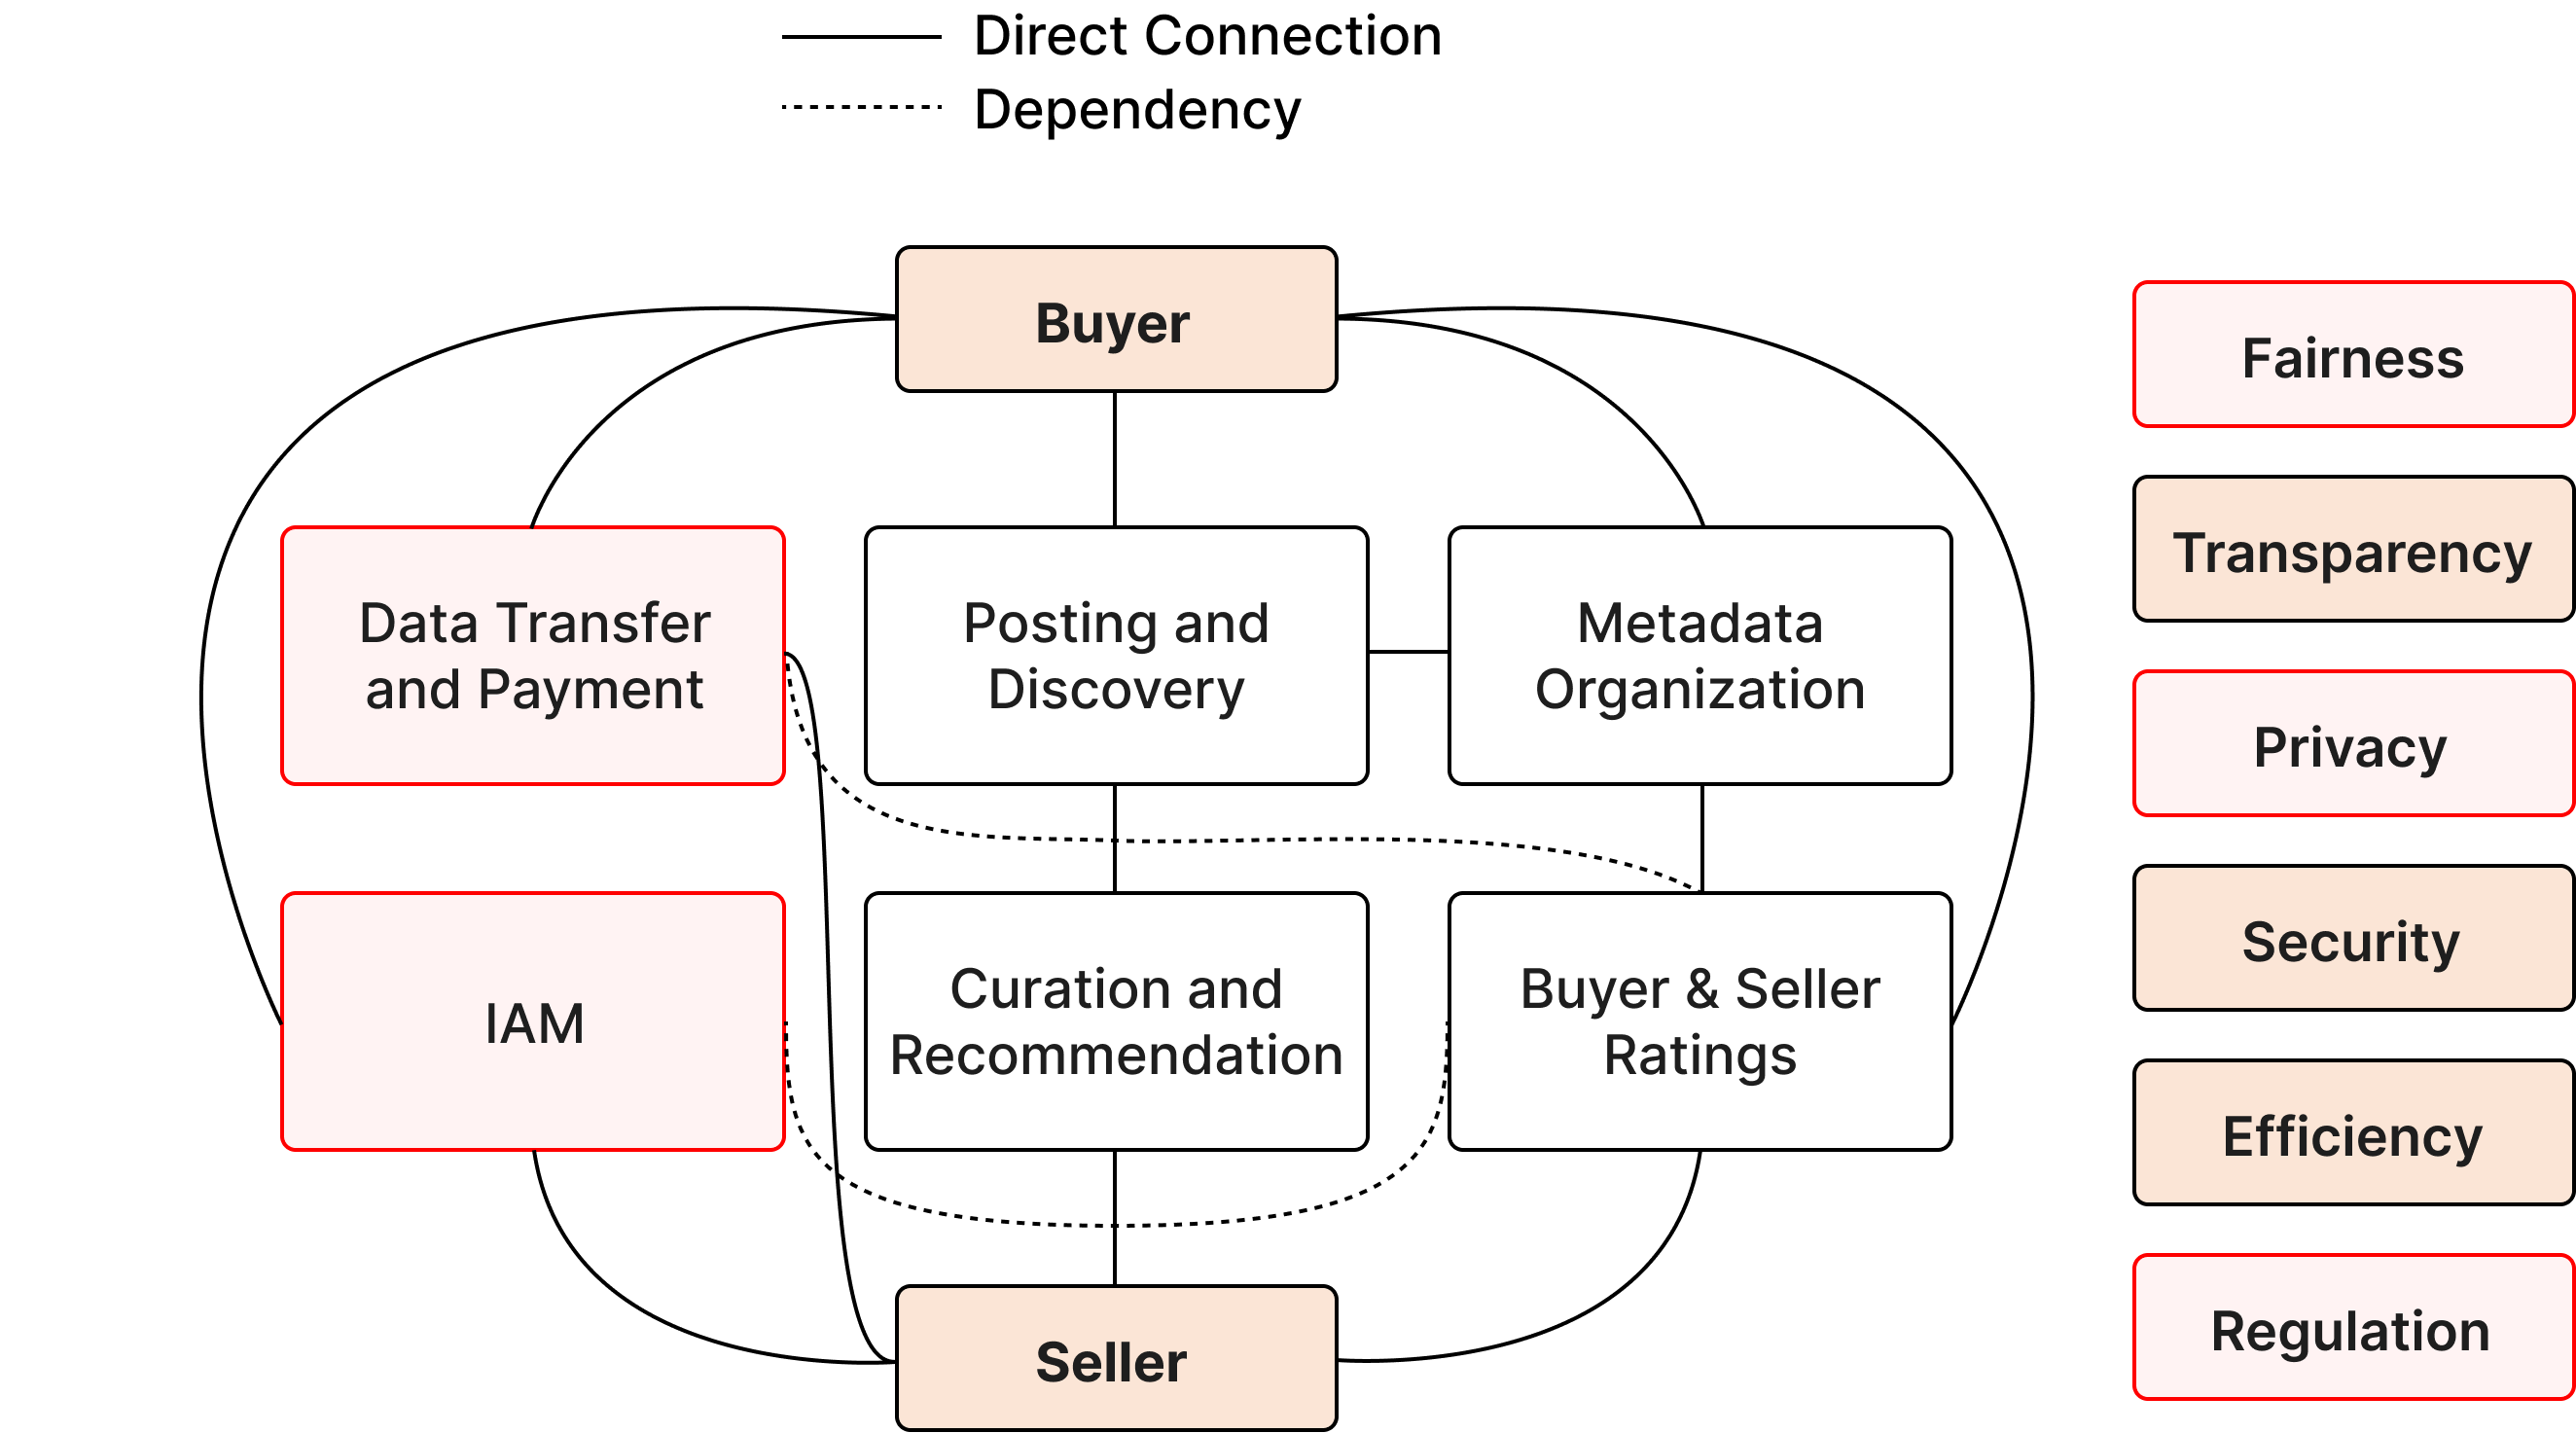
\includegraphics[width=13cm]{images/components.png}
%    \caption[Key components and features of a digital data trading platform]{Key components and features of a digital data trading platform. All components in red show the aspired enhancements by the contributions of this thesis.}
%    \label{fig:components}
%\end{figure}

%"Blockchain-based application architectures benefit from a set of unique properties including immutability and transparency of cryptographically-secured and peer-recorded transactions, which have been agreed upon by network consensus" \cite{eberhardtBlockchainInsightsOffChaining2017}. According to that, it is trivial to implement sufficient \emph{Transparency} and \emph{Security} in blockchain-based data marketplaces. Furthermore, it turns out the non-trivial \emph{Fairness} problem in a two-party trading relationship seems to be solved by Blockchain technology in one atomic swap \cite{dziembowskiFairSwapHowFairly2018,liZKCPlusOptimizedFairexchange2021}. However, \emph{Privacy}, \emph{Regulation} and \emph{Efficiency} remains a bigger problem for blockchain-based data marketplaces due to limitations of public permission-less Blockchains such as Bitcoin \cite{nakamotoBitcoinPeertoPeerElectronic} and Ethereum \cite{buterinNEXTGENERATIONSMART}.

%Public permission-less Blockchains inherently validate and process transaction data at every node, in order to guarantee network consensus. By virtue of its design, all data is available at each node which makes this system purposely public in favor of transparency properties. However, data sharing often incorporates \acrfull{pii} and confidential data. Consequently, storing and computing private data on these ledgers is conflicting with Privacy requirements, enforced by regulations such as the \acrfull{gdpr} \cite{european_commission_regulation_2016}. In any case, it is not advisable to store large amounts of data in Blockchains due to block-size limitations, Blockchain bloating and extremely high associated storage costs.

%Off-chain storage solutions are suggested to overcome this limitation. In particular the Content-Addressable Storage Pattern \cite{eberhardtBlockchainInsightsOffChaining2017} seems to be a reasonable solution to store large amounts of data while keeping key properties of Blockchains such as immutability. Decentralized peer-to-peer networks such as IPFS \cite{benetIPFSContentAddressed2014}, Filecoin \cite{filecoin} and SWARM \cite{swarm} provide a promising approach to that. However, these networks suffer from the same Privacy issues as Blockchains due to open access and data replication across the network.

%Another problem seems to be the enforcement of access and usage regulations in a distrusted setting without a \acrfull{ttp}. A seller loses full control over his data when the buyer receives it. Hence, he or she is not able to enforce geographical usage restrictions or purpose limitations for example. This especially violates the principle of purpose limitation codified in Art. 5 of the \acrshort{gdpr} \cite[Art. 5 (1 b)]{european_commission_regulation_2016}. Given a malicious buyer, he or she might even resell the purchased dataset without the seller's knowledge.

No matter if centralized or decentralized infrastructure, it is observable that most problems occur when data leaves the boundaries of the seller, i.e. raw datasets are moved to an intermediate storage platform and/or the buyer, to be processed. In a naive approach, sellers would encrypt raw datasets in the first place, however, \emph{Ownership}, \emph{Privacy}, and \emph{Regulation} still remain a problem, once they are decrypted by the buyer or the buyer loses decryption keys. Accordingly, we suggest flipping the strategy, i.e. raw datasets never leave the boundaries of the seller, such that only a computation over the dataset is moved to the buyer, thereby protecting \acrshort{pii} and confidential data. This paradigm is referred to as \emph{\acrfull{c2d}}. However, a problem with this paradigm is that, given a malicious seller, the buyer cannot verify if the result has been computed correctly. \acrfull{voc} has been suggested to address this problem \cite{eberhardtBlockchainInsightsOffChaining2017,eberhardtOffchainingModelsApproaches2018}.

% im gegensatz zu physical goods haben daten nur wert wenn sie korrekt sind!!!!!!!!!!!!!!!

%Verifiable Off-chain Computation (VOC) has been suggested to address this problem \cite{eberhardtOffchainingModelsApproaches2018,eberhardtBlockchainInsightsOffChaining2017}.

%This thesis focuses on \emph{Privacy}, \emph{Fairness} and \emph{Regulation} enhancements in blockchain-based data trading platforms, by combining Compute-to-Data with Verifiable Off-chain Computation (VOC). It implicitly targets the \emph{Data Transfer} and \emph{Payment} process as well as \emph{IAM} -- some of the fundamental functional requirements, as depicted in Figure \ref{fig:components}.

%Thereby, we make two individual contributions ...:

This thesis presents a practical real-world implementation of a blockchain-based data marketplace for verifiable computations on private datasets. Accordingly, buyers can discover interesting datasets on the marketplace and purchase arbitrary computations such as an average of some hidden data records. Sellers instead are responsible for executing those computations within their boundaries and for submitting the result along with a verifiable proof of computational correctness. Thereby, the proposed solution enhances \emph{Ownership}, \emph{Privacy}, and \emph{Regulation} in blockchain-based data trading platforms with a focus on static infrequently changing datasets as opposed to real-time streaming data and training of machine-learning models. Specifically, this thesis leverages \acrshort{voc}, in particular a \acrfull{zkp} protocol, implemented with the ZoKrates\footnote{https://github.com/Zokrates/ZoKrates} toolbox, to cryptographically prove computational correctness on the Ethereum blockchain. Besides that, blockchain technology is used (i.) to process payments; (ii.) to create a transparent, non-repudiable, and tamper-proof log of events; (iii.) to enforce data usage policies.  
%It specifically targets the \emph{Data Transfer} process between buyer and seller -- one of the fundamental functional requirements in a data marketplace.

%weitere problems je nach art des marketplaces
\begin{enumerate}
    \item What components are mandatory for a blockchain-based data marketplace and how can the \acrlong{c2d} paradigm be applied?
    \item How can the \acrlong{c2d} paradigm be made verifiable without sacrificing ownership, privacy and regulation?
    \item How practical is the proposed solution?
\end{enumerate}

The remainder of this thesis is organized as follows: Chapter \ref{cha:background} provides fundamental background knowledge to understand the remainder of this thesis. Chapter \ref{cha:relatedwork} gives a brief overview of the current research, with regard to privacy-aware blockchain-based data marketplaces. Chapter \ref{cha:requirements} summarizes the functional and non-functional requirements for the desired software artifact outcome. The concept \& design of the software artifact is outlined in Chapter \ref{cha:cod} and its implementation is explained in Chapter \ref{cha:implementation}. Lastly, Chapter \ref{cha:evaluation} evaluates and discusses the implementation based on the defined requirements, followed by a conclusion in Chapter \ref{cha:conclusion}, to summarize the results and ideas for future work.


% https://ieeexplore.ieee.org/stamp/stamp.jsp?arnumber=9739681
%Compute-to-data has already been discussed as an access
%method in section III-A, but it is also a solution that addresses
%problems of transaction enforcement, as well as maintaining
%data governance. With compute-to-data, rather than handing
%over the data to the data consumer for consumption in their
%environment, the consumer sends code to manipulate the data
%and receives results of computation that generally do not
%expose the underlying data. In its simplest form, the data
%provider sends the code directly to the data provider, who
%either provides an environment for execution of the code
%or runs the code manually themselves [19], [52]. However,
%since code can also be considered a data product, the data
%consumer might not be willing to share their code for the
%same reasons the data provider is not. In such a case, a trusted
%third party can be charged with providing an isolated environment where the code can be executed on the data [31], [34].
%A special case of compute-to-data is the use of multi-party
%computation whereby code is run on multiple data products
%in multiple physical locations, and an aggregate result is
%obtained without revealing information from the individual
%data products [147].

% dataset: https://archive.ics.uci.edu/ml/datasets/daily+and+sports+activities#
% https://archive.ics.uci.edu/ml/datasets.php
\chapter{Background}
\label{cha:background}

\chapter{Related Work}
\label{cha:relatedwork}

Blockchain-based data trading platforms have been researched for a long time. There are various approaches where blockchains are used (i.) as a transparent tamper-proof log of events and immutable link to an asset; (ii.) as an enforcement point for access control decisions; (iii.) as a medium to ensure fair exchange; and (iv.) as a highly secure and available infrastructure. However, the degree of privacy, ownership, fairness, and regulation is very different among those implementations. Therefore, various off-chain components were proposed on top of the blockchain to improve these properties.

% data quality

% also asymmetric key with public key infrastructure to encrypt plaintext and decrypt ciphertext?https://cpl.thalesgroup.com/faq/key-secrets-management/what-asymmetric-key-or-asymmetric-key-cryptography

% ramachandranDecentralizedDataMarketplace2018 - rating system to ensure trust
% banerjeeBlockchainEnabledData2019 - encryption and zkp, homomorphic encryption could be added, data leaves boundaries -> our approach not
% truongSecureDecentralizedSharing2019 - private blockchain hyperledger, data stored in cloud but encrypted before

% bisschen mehr auf blockchain eingehen + alle anderen properties, weniger fairness

In the most straightforward implementation \cite{ozyilmazIDMoBIoTData2018,banerjeeBlockchainEnabledData2019}, sellers use a symmetric key to encrypt datasets before they are stored or transferred to the buyer. This protects the dataset's privacy and weakens trust assumptions on any intermediary storage platform. Decryption keys are then distributed securely to the buyer after purchasing a dataset. Truong et al. \cite{truongSecureDecentralizedSharing2019} rely on encrypted datasets as well, however, with a more sophisticated key-distribution scheme. Accordingly, prefix encryption, as a form of Hierarchical Identity-Based Encryption (HIBE), links the decryption key to an identity, simplifying key distribution and allowing fine-grained access control. Nevertheless, both approaches lack privacy and regulation as soon as the dataset is decrypted. Our proposal has end-to-end privacy by default without encryption, such that only a computed result of the raw dataset leaves the boundaries of the seller. 

Serrano and Cuenca \cite{serranoPeertoPeerOwnershipPreservingData2021} enhance data ownership, privacy, and regulation with \acrfull{he}. According to that, buyers can perform arbitrary computations on encrypted datasets, while the result is decrypted by the seller. Hence, raw datasets never leave the boundaries of the seller. While this is another valid approach to a Compute-to-Data paradigm it severely lacks output verifiability, introducing higher trust assumptions in all participants to act honestly. Our approach requires no trust since computations are cryptographically verifiable on the blockchain due to \acrshort{zkp}'s. A different approach is followed by Enigma \cite{shrobeEnigmaDecentralizedComputation2018} which uses \acrfull{smpc} for data queries with guaranteed privacy by design. With \acrshort{smpc}, every party in the protocol has only access to a meaningless piece of data, whereas only the buyer finally receives the result of the computation. Enigma even uses cryptographic proofs on the blockchain to enable public output verifiability and security deposits to incentivize honest behavior. Unlike our approach, Enigma needs a significant amount of computing nodes to make the system entirely secure. Our marketplace instead could potentially work with one buyer and one seller node.

Dai et al. propose another Compute-to-Data paradigm with a secure data trading ecosystem \cite{daiSDTESecureBlockchainBased2020} for statistical queries and aggregations on private datasets. Ownership, privacy, and correct computation of the dataset are ensured in a \acrfull{tee}, specifically using Intel’s Software Guard Extension (SGX) enclaves. Hynes et al. \cite{hynesDemonstrationSterlingPrivacypreserving2018a} as well as Xiao et al. \cite{xiaoPrivacyGuardEnforcingPrivate2020} follow similar approaches, while the latter adds (i.) a novel way to commit the computation result to the blockchain; and (ii.) a verifiable proof to show compliance to data usage policies as a consumer. However, all approaches require special \acrshort{tee} compatible hardware, and \acrshort{tee}'s have been shown to be susceptible to side-channel attacks \cite{brasserSoftwareGrandExposure,biondoGuardDilemmaEfficient}.

One of the most privacy-preserving approaches is followed in \cite{fotiouPrivacypreservingStatisticsMarketplace2021} by Fotiou et al. with a computation result based on \acrfull{dp}. "\acrshort{dp} addresses the paradox of learning nothing about an individual while learning useful information about a population" \cite{tsaloliDifferentialPrivacyMeets}. This implicitly introduces an error margin into the computation result. However, this paper does not implement output verifiability. Albeit, \cite{narayanVerifiableDifferentialPrivacy2015,tsaloliDifferentialPrivacyMeets,koutsosAgoraPrivacyAwareData} show that output verifiability with \acrshort{dp} is possible by the use of \acrshort{zkp}'s.

%agora
%Data privacy: no party can learn any information about the
%raw data of the generators, apart from the function output
%that is learnt by the broker and paying consumers.
%Output verifiability: no broker can successfully sell an incorrect
%or falsified result to a consumer.
%Atomicity of payments: no entity can avoid paying for services,
%i.e., generators are reimbursed for their data and
%brokers are paid for providing function outputs.
\chapter{Requirements}
\label{cha:requirements}

The following functional and non-functional requirements define what the designed marketplace should be capable of, in the scope of this thesis, and what should be its general properties. Thereby, each requirement is classified in Table \ref{tab:nfr-vs-fr} according to its type and explicitly numbered to be used as a reference. Furthermore, each requirement is described as a user story to be easily understandable, to focus on business values and the customer's needs, and to support iterative development in an agile way. Those user stories are very coarse-grained and thus refined into specific development tasks, as visible on our KanBan\footnote{https://github.com/users/amrap030/projects/1} board. Non-functional requirements are not visible on the board, because they are general properties that translate into each functional requirement when implemented.

% scalability missing? would be 8th nfr -> then +1 fr?
% verification als fr?
% fairness und efficiency rausnehmen? tos rausnehmen?

\begin{xltabular}{\textwidth}{lllX}
\toprule
\textbf{\#} & \textbf{Type} & \textbf{Name}   & \textbf{Description} \\ \midrule
\endfirsthead

\multicolumn{4}{c}%
{\tablename\ \thetable{} -- continued from previous page}\vspace{2mm} \\
\endhead
    F01 & Functional & Sell datasets & As a seller, I would like to sell valuable datasets in a privacy-preserving manner, so that I get compensated for data access by interested parties to make a profit. \\ \midrule
    F02 & Functional & Search datasets & As a buyer, I would like to explore the marketplace by full-text search or tags, so that I find interesting datasets more quickly. \\ \midrule
    F03 & Functional & Filter datasets & As a buyer, I would like to filter datasets when exploring the marketplace so that I reduce the offers to a minimum to find interesting datasets more quickly. \\ \midrule
    F04 & Functional & Buy computations & As a buyer, I would like to buy a computation on a dataset to perform data analytics to gain new insights on interesting datasets. \\ \midrule
    F05 & Functional & Create algorithms & As a marketplace participant, I would like to create computing algorithms so that buyers can use them to compute data. \\ \midrule
    F06 & Functional & Check quality & As a buyer, I would like to check the data quality before I buy a computation so that the result is not falsified. \\ \midrule
    F07 & Functional & Create ToS & As a seller, I would like to declare terms of use for data usage, so that any misusage is punishable. \\ \midrule
    N01 & Non-Functional & Privacy & As a seller, I would like to protect \acrshort{pii} and confidential data in my raw datasets, so that buyers learn nothing more than the result of a computation on a never seen private dataset. \\ \midrule
    N02 & Non-Functional & Ownership & As a seller, I would like to preserve ownership of my raw datasets, so that nobody else can make use and profit from my own dataset. \\ \midrule
    N03 & Non-Functional & Fairness & As a marketplace participant, I would like to encounter fair exchange, so that buyers receive legitimate data while sellers receive the agreed-upon payment without cheating. \\ \midrule
    N04 & Non-Functional & Security & As a marketplace participant, I want the marketplace to have a secure information exchange and to be resilient against malicious attackers and unauthorized access.   \\ \midrule
    N05 & Non-Functional & Efficiency & As a marketplace participant, I want the interaction with the marketplace to be at a comparable speed to state-of-the-art marketplaces so that I don't get frustrated when using it. \\ \midrule
    N06 & Non-Functional & Transparency & As a marketplace participant, I want to have all events on the marketplace be publicly traceable, so that trust and compliance are increased in the marketplace.  \\ \midrule
    N07 & Non-Functional & Availability & As a marketplace participant, I want the marketplace in its entirety to be available 99.99\% of the time I try to interact with it so that I can make a purchase, search or sell data when needed. 
    \\ \bottomrule
\caption{TODO TODO TODO!} \label{tab:nfr-vs-fr}
\end{xltabular}%

\chapter{Concept \& Design}
\label{cha:cod}

This thesis presents the implementation of a practical real world data marketplace for verifiable statistical computations on private datasets. It addresses \emph{Privacy}, \emph{Fairness} and \emph{Regulation} problems of blockchain-based data trading platforms, while the focus is on \emph{Privacy}. \emph{Furthermore, I only focus on static tabular datasets with very infrequent changes. Hence, I do \textbf{not} focus on real-time streaming data and training of machine-learning models}. My proposed implementation implicitly targets the \emph{Data Transfer} and \emph{Payment} process as well as \emph{IAM} -- some of the fundamental functional requirements, as already depicted in Figure \ref{fig:components}. Specifically, I construct a secure blockchain-based data trading ecosystem, using Blockchain as a medium to (i.) prevent single-point of failure; (ii.) define data usage policies; (iii.) create a transparent, non-repudiable and tamper-proof log of transactions; and (iv.) enforce a fair data exchange protocol. However, the \emph{focus} of this thesis is rather on creating a generic mechanism to make a variety of computations on arbitrary private datasets verifiable, and Blockchain is a necessary part of the puzzle. This thesis uses Verifiable Off-chain Computation (VOC) to address this problem \cite{eberhardtOffchainingModelsApproaches2018,eberhardtBlockchainInsightsOffChaining2017}.

VOC is a derivative of Verifiable Computation and aims to secure the integrity of computations performed by untrusted parties off the Blockchain. The result of the computation is then published to the Blockchain and verified on-chain with a cryptographic proof, attesting its correctness. Off-loading the computation has multiple benefits -- (i.) it increases the scalability by avoiding complex redundant computations on each node; (ii.) it reduces on-chain transaction costs by significantly lowering the size of transactions; and (iii.) it improves privacy by hiding PII and confidential data from the public ledger. \cite{eberhardtOffchainingModelsApproaches2018,eberhardtZoKratesScalablePrivacyPreserving2018a,simunicVerifiableComputingApplications2021,xuSlimChainScalingBlockchain} 

According to \cite{eberhardtOffchainingModelsApproaches2018}, a reasonable VC scheme for off-chain computations needs to fulfill the following requirements: (i.) non-interactivity; (ii.) cheap verification; (iii.) weak security assumptions; and (iv.) zero-knowledge. ZkSNARKs, ZkSTARKs and Bulletproofs provide a valid approach to the aforementioned requirements. ZkSNARKs are a type of Zero-knowledge proof (ZKP) that are \emph{non-interactive} and \emph{succinct}. \emph{Non-interactivity} defines the possibility to convince a verifier of a particular statement with only \emph{one} message \cite{eberhardtOffchainingModelsApproaches2018,eberhardtZoKratesScalablePrivacyPreserving2018a,simunicVerifiableComputingApplications2021}. \emph{Succinct} defines a proof that is small in size, compared to ZkSTARKs and Bulletproofs, and can be verified cheaply and quickly, typically within a few milliseconds \cite{simunicVerifiableComputingApplications2021}. This thesis uses a ZKP with ZkSNARKs for verifiable computations on private datasets.

The proposed blockchain-based data trading platform is designed for two party relationships between a buyer \emph{B} and seller \emph{S}. The current high-level protocol for a trade between \emph{B} and \emph{S} on the proposed platform is described by the following exemplary use case and shown in the subsequent Figure \ref{fig:usecase}, without technical details.

\begin{figure}[!htb]
    \centering
    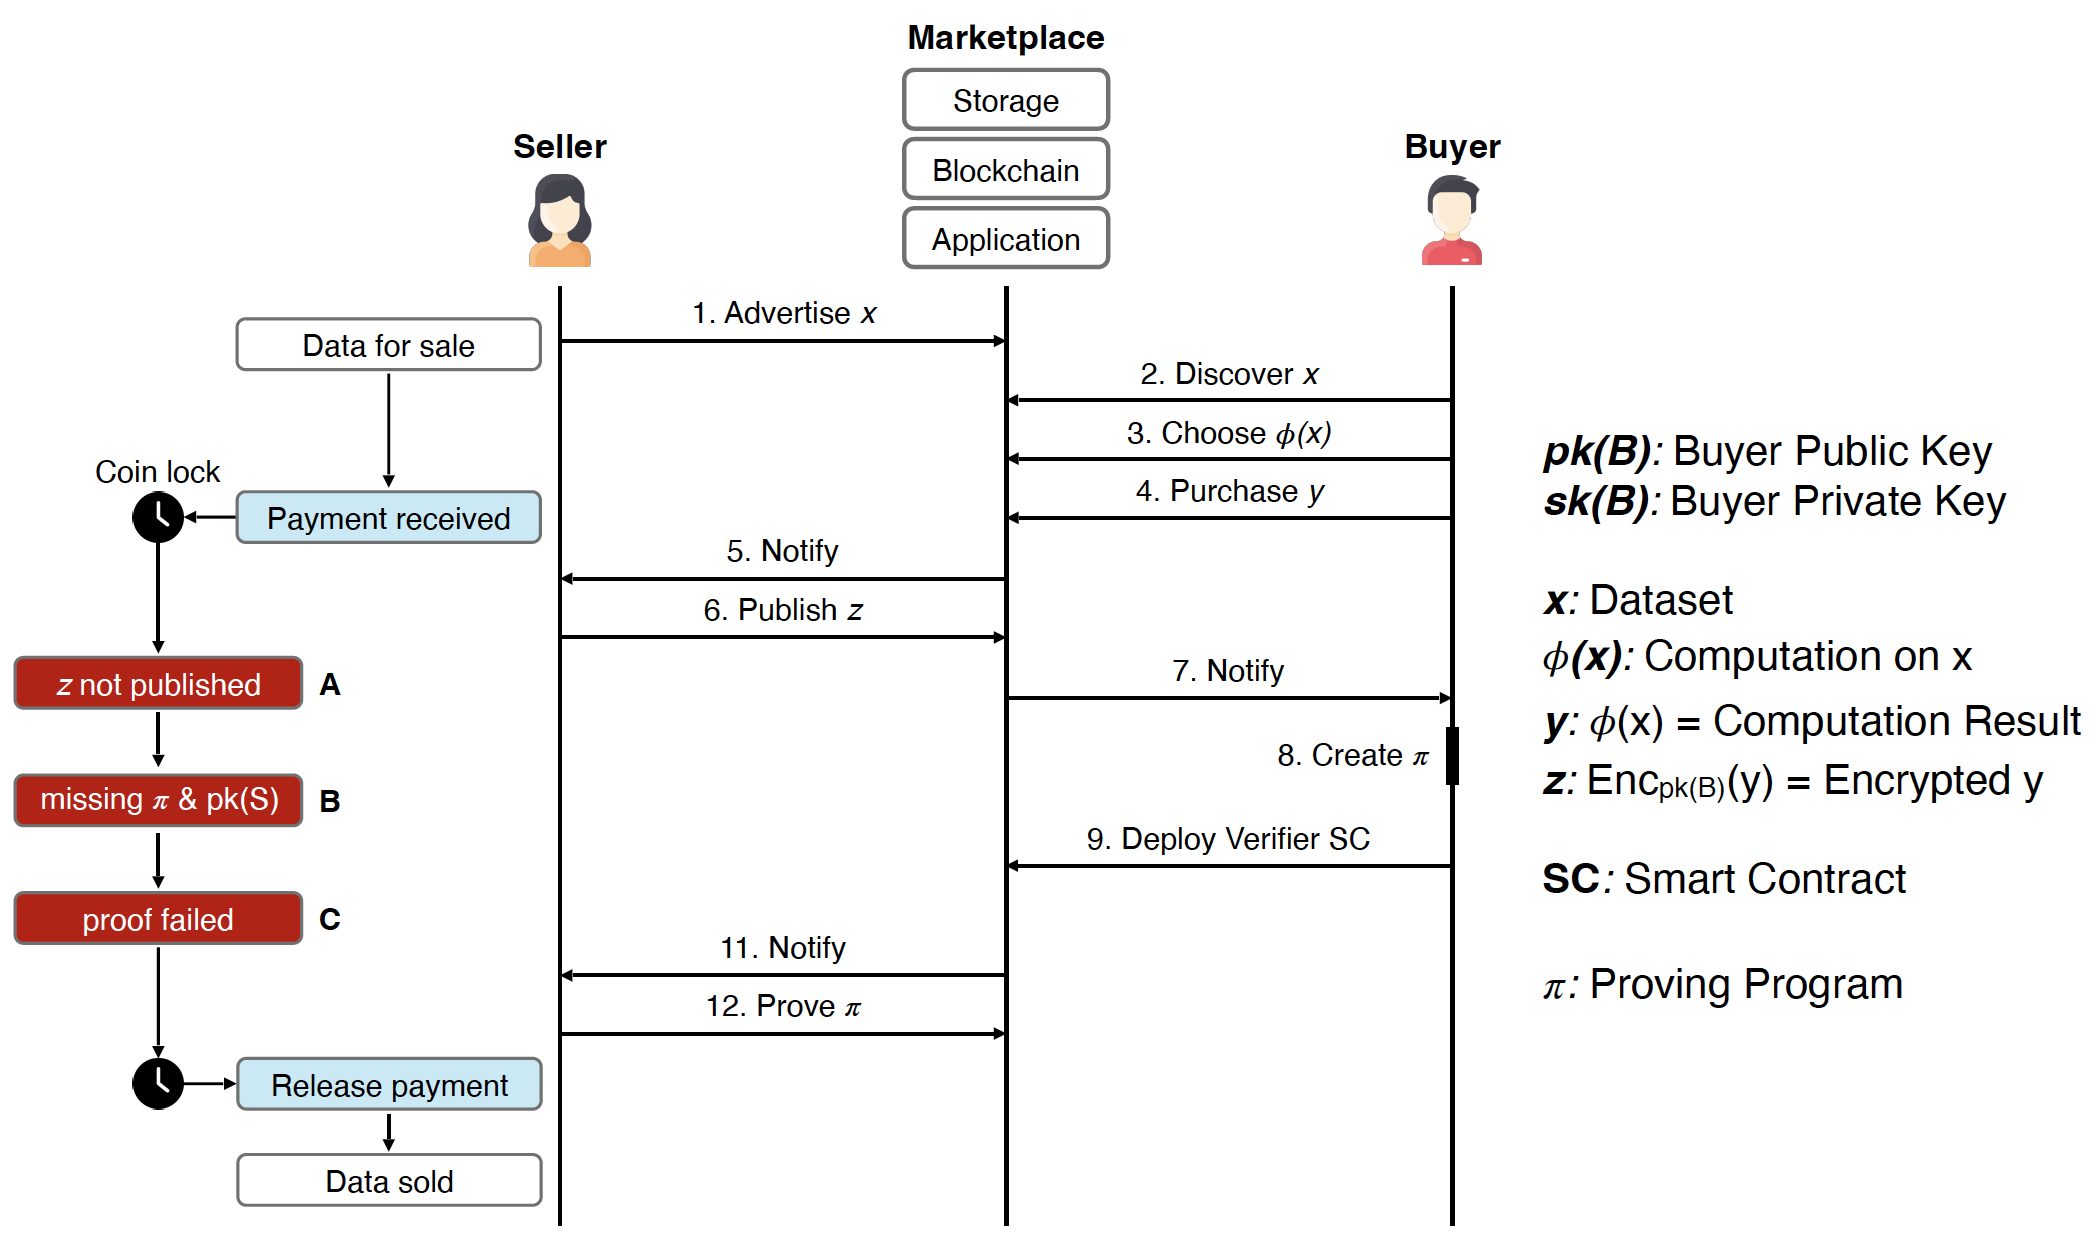
\includegraphics[width=14cm]{images/protocol.png}
    \caption{Proposed protocol for a blockchain-based data trading platform with Compute-to-Data and Verifiable Off-chain Computation for verifiable statistical queries on private datasets. The marketplace between a buyer \emph{B} and seller \emph{S} is highly abstracted into storage, Blockchain and application components, which are necessary for the entire data marketplace ecosystem.}
    \label{fig:usecase}
\end{figure}

\subsubsection{Example}

S advertises a dataset $x$ about health information of a population on the marketplace. The dataset $x$ is described by metadata, i.e. the time interval, data category, amount of columns and rows as well as the header of each column, among other metadata. The actual content of the dataset is hidden from the buyer. A potential \emph{B} enters the data marketplace and is interested in receiving the average age of cancer diagnosed patients in 2021. He or she discovers a promising dataset $x$ of \emph{S} in the health category, containing all cancer diagnosed patients worldwide. \emph{B} chooses to purchase the desired computation $\phi(x)$ for the \emph{age} column. He or she commits the purchase by an on-chain transaction, including the given price by \emph{S}. All coins are now temporarily locked in a smart contract. \emph{S} subsequently gets notified by the purchase and calculates the average on a private node of \emph{S}, protecting privacy and confidentiality of \emph{S}'s dataset. \emph{S} transfers the result $z = Enc_{pb(B)}(y=\phi(x))$ to the Blockchain, encrypted with the public key of \emph{B}. \emph{B} gets notified and decrypts the result with his or her private key $Dec_{sk(B)}(z)$. \emph{B} is now uncertain about the correctness of the result and therefore constructs a program $\pi$ for the seller to prove (i.) the correctness of the computation; (ii.) the result originates from the advertised dataset; and (iii.) the proof is given by the seller. He or she then publishes a smart contract for the verification of the proof. \emph{S} is now responsible to generate such a proof for the verifier smart contract, to transparently proof all the requirements of $\pi$. According to that, the execution of the protocol terminates in the following situations:

\newpage
\begin{enumerate}
    \item \emph{S} finally manages to submit a valid proof to the verifier contract. In this case, the payment is released to \emph{S}.
    \item \emph{S} does not publish a computation result. In this case, \emph{B} can withdraw his payment after a timeout. \textbf{(Scenario A)}
    \item \emph{B} does not construct a proving program and does not publish the proving key to \emph{S}. In this case, \emph{S} can withdraw the payment after a timeout. \textbf{(Scenario B)}
    \item \emph{S} is not able to submit a valid proof to the verifier contract. In this case, \emph{B} can withdraw his payment after a timeout. \textbf{(Scenario C)}
\end{enumerate}

\noindent \textbf{Note}: This protocol is only a first idea and the final protocol may highly differ. At the time of writing this exposé I already noticed that there is one major weakness in the current protocol. A malicious \emph{B} could send a fake proving key to \emph{S}, so that it is impossible for \emph{S} to construct a valid proof. According to that, \emph{B} would always be able to withdraw his payment, if he has no honest interest in actually verifying the correctness of his purchased values. While this is not the focus of this thesis, I will try to create a completely trustless protocol between \emph{B} and \emph{S}.
\chapter{Implementation}
\label{cha:implementation}

The final outcome of this thesis will consist of multiple software artifacts, implementing a fully functional data marketplace, as described in the use case of the previous chapter \ref{chapter:solution}. The combination of all software artifacts builds the blockchain-based data trading platform. According to that, the platform is composed of a public permissionless Blockchain, a Blockchain Indexer, a Marketplace User Interface, a decentralized Off-chain Storage Node, a private Compute Node and a Zero-knowledge Proof Service. 

\subsubsection{Blockchain}
The Blockchain is the single source of truth for all advertised datasets on the the marketplace user interface. It provides non-repudiable tamper-proof logs of transactions, everything visible via the user interface. All necessary smart contracts will be written using the Solidity\footnote{https://github.com/ethereum/solidity} programming language and deployed to an Ethereum Virtual Machine (EVM) compliant public permissionless Blockchain such as Ethereum itself, or a layer 2 network such as Polygon. 

\subsubsection{Blockchain Indexer}
Unfortunately, the Blockchain is a time-ordered append-only data structure, which makes it highly inefficient to query, i.e. filter, search, paginate and aggregate. However, for a practical data marketplace this is absolutely necessary. Blockchain Indexers typically provide an efficient protocol, to extract raw data from the Blockchain, process it and store it into some kind of database, as soon as a new block is written to the ledger. Additionally, Blockchain Indexers expose an API, to provide highly efficient and fast access to Blockchain data with all desired querying capabilities. The Blockchain indexer will be implemented with the Graph\footnote{https://thegraph.com/en/}.

\subsubsection{User Interface}
The user interface is the entry point to the blockchain-based data trading platform. A seller can advertise and monetize arbitrary datasets whereas a buyer can transparently browse the marketplace and buy interesting datasets. It will provide most of the functional requirements of Figure \ref{fig:components} and will be implemented as a Vue\footnote{https://vuejs.org/} 3 single page application (SPA) with commonly used libraries such as Ethers.js\footnote{https://github.com/ethers-io/ethers.js/} and Hardhat\footnote{https://github.com/NomicFoundation/hardhat} to efficiently build modern decentralized applications (dApps). To securely interact with smart contracts, I will use Metamask\footnote{https://metamask.io/} as a wallet.

\subsubsection{Off-chain Storage}
The off-chain storage node is not used to store the advertised raw datasets. It is rather used to store the dataset's metadata according to the Content-Addressable Storage Pattern\cite{eberhardtBlockchainInsightsOffChaining2017}, including a detailed description of the dataset and its hash. As a decentralized peer-to-peer storage network, the InterPlanetary File System\footnote{https://docs.ipfs.tech/} (IPFS) will provide highly available and immutable access to metadata. A content identifier (CID) is stored with every advertised dataset on-chain.

\subsubsection{Compute Node}
The compute node is a private node of the seller to fulfill the purchase order of the buyer, i.e. computing a statistical query on a private dataset. This compute node will be implemented as a Node.js\footnote{https://nodejs.org/en/} application.
%- policies
%- purpose based access control + abac

\subsubsection{Zero-knowledge Proof Service}
The ZKP service is the focus of this thesis and will automatically generate proving programs based on the individual purchase of a buyer. It compiles high-level ZoKrates\footnote{https://github.com/Zokrates/ZoKrates} code into an executable constraint system (ECS) using the Intermediate Representation (ZIR) of ZoKrates. Furthermore, it automatically generates an evidence key pair for proof creation and verification, also referred as the one-time setup. Finally, a buyer can send the proving key to the seller and deploys a smart contract for proof verification. The seller uses the proving key and the generated proving program to deliver such a proof.
\chapter{Evaluation}
\label{cha:evaluation}

The outcome of this thesis will be evaluated according to predetermined functional and non-functional requirements. As already described in the previous sections, this thesis aims to enhance \emph{Privacy}, \emph{Fairness} and \emph{Regulation} in blockchain-based data trading platforms by combining Compute-to-Data and Verifiable Off-chain Computation. These 3 requirements are hard to measure numerically, but the evaluation will include an in-depth discussion about the pros and cons of the proposed system design accordingly, and compared to related work. %However, if I manage to implement verifiable Differential Privacy, privacy gets indeed measurable. % Possibly in form of Threat Model?

The second part of the evaluation will include multiple benchmarks with regards to the practicality, also referred as efficiency, of the proposed system design. Interestingly, \emph{Efficiency} is one of the key features of any digital data trading platform as depicted in chapter \ref{chapter:problem}. %Hence, the result of this evaluation will provide a decent proposition about the real 
Therefore, I will analyze efficiency of on-chain and off-chain components individually, according to costs, scalability and computation time.

One of the most suitable measurements for on-chain components are the costs for each transaction, with regards to gas fees. This is important because the proposed system design is only feasible as a real-world system when costs are reasonably low for the buyer and seller. Since the Blockchain is primarily used to secure the protocol, costs can be compared to conventional buyer and seller protection systems from Ebay or PayPal for example. The most important on-chain transaction will probably be the verification of the zero-knowledge proof, which has to be cheaper than the on-chain execution in the first place. Benchmarks will vary in the size of the dataset and the computation algorithm.

The second analysis includes the evaluation of off-chain components. According to that, the ZKP, which is composed of different phases, is the most important evaluation. I will benchmark especially the time for the one-time setup as well as the proof generation time. The proof generation time will probably have the most impact on the practicality of the proposed system design. Benchmarks will again vary in the size of the dataset and the computation algorithm. Furthermore, I will take the underlying hardware with regards to the computational power into account for this analysis. 

The entire system can be measured in the overall time and amount of exchanged messages until the trade between buyer and seller is completely fulfilled. All benchmarks can be compared to conventional data marketplaces as well as related work, and used to construct suggestions to improve the system design in future work.

THREAT MODEL?
\chapter{Conclusion}
\label{cha:conclusion}


%--------------------------------------------------------------
% TABLES, FIGURES, BIBLOGRAPHY AND APPENDICES
%--------------------------------------------------------------
\backmatter

% Lists of tables and figures
\listoftables
\listoffigures
\printglossary[type=\acronymtype,title={List of Abbreviations}]
\addcontentsline{toc}{chapter}{List of Abbreviations}
\lstlistoflistings

% Bibliography
\setwidesite{}						% Set page to be wider for bibliography
\markboth{Bibliography}{bibliography}
\label{cha:bibliography}
\bibliographystyle{IEEEtran}
\bibliography{bibliography.bib}

% Use following to separate online (websites) and offline (books, papers) sources
%\printbibliography[heading=offline,filter=offline]
%\printbibliography[heading=online,filter=online]

%\begin{appendices}
%	\chapter{Appendix 1}
\label{appendix:listing1}

\lstset{language=PHP}
\begin{lstlisting}
for($i=1; $i<123; $i++)
{
    echo "work harder! ;)";
}
\end{lstlisting}
	% \input{content/99_appendices/a02_listings}
	% \input{content/99_appendices/a03_listings}
%\end{appendices}

\end{document}
